\documentclass{article}
\usepackage[UTF8]{ctex}
\usepackage{graphicx}
\begin{document}
\renewcommand\title[1]{\par\vspace*{2ex}\centerline{\large#1}\par}
\renewcommand\date[1]{\par\hfill#1}
\section{高三段}
\title{望柳}
看茂盛的柳树,想到腹中的学问。柳条不计其数,学问却有限,怎样才能使自已的知识如柳条那样多,那样有条理呢?柳树一点一点地从小树长成大树,从一枝长成万枝,从几叶长到无数,难道仅仅是一天一天,一年一年的结果吗?不知它使了多少力气,吃了多少苦头,才使人赏心悦目、赞叹不已。要想同那柳树一般茂盛,怎能坐着等待,走着幻想呢。必须日积月累,毫不松懈才行啊。
\title{解题}
解题不为解,为其中的知识,为使用的方法,更为那宽广的思想。习其知识,温其方法,感其思想,以此求熟。析丝缕以劳心,辨是非以用智。心越用越灵,智越用越明。于是解题之用更显,而解题之趣存矣。若只为解题,乐其功,惧其败,则功败渐难动心而趣失矣。不若多费心智而趣无尽也。故解题求熟之道,不可只求解,须更辛苦也。
\title{雪}
今天中午,我去餐厅的路上看见一只死鸟,脚不停步走了过去。觉得不对。又听见别人厌恶地说:这儿有个死鸟。更觉得不好。便回去慢慢地捡起它,扔在大花坛里,然后去吃饭。

夏日夜里许多蟋蟀飞到班级里,被人踩死了很多,经常看到死蟋蟀泥身是泥,缺头少腿十分可怜。我时常捡起它们来,扔到有土的地方去。今天,那只鸟,睁着眼,张着又长又黄的嘴,就像夏日可怜的蟋蟀,死在水泥地上,被当作拉圾,是多么可怜的啊!
\title{尺子}
物理课讲到光学,老师带尺子来上课。老师画线很直,还用尺子画直线,我画得不直,更不能单手作图。老师说图要画准,不用尺子不行。她用尺子,我不会不用。
\title{自我介绍}
\small 我拾筷子使其归食堂,既夸我又要表扬,将为我申请奖学金而使我介绍家庭情况,我作文并抄下:
\normalsize\par
名叫王崇宁,家在民权县龙塘镇黄庄村。村子虽大,我家普通,房子四间,家人四口,父母无业,田只一人。我的父亲去陕西挣钱,去年染病,叫出血热。住院一两月,在家闲半年,至今力气少,腰痛常贪床。我的母亲去外地挣钱,先往新疆,后到天津,又去陕西。大前年夏祖母被查出肉瘤,母亲不能外出,况且始终多病,那时胃疾,这时臂痛。信仰耶稣,从我儿时起。在家里母亲教我识数字,小学父母管得严,中学经常问我学习的事情。高中二年级在第二十一班,徐兰老师作班主任,同学努力,我常恐怕作业太多。曾奋力做题,致头脑混乱,从床上滑下去,摔伤了腿。有些作业不能完成。追求知识,熟练应用。学习成绩排名五百。我爱护公物,看见扫帚头把分离而修理,看见有人拧掉水龙头却不敢问。那掉在地上的筷子,越踩越脏;那弃在操场上的筷子,越久越糟,可不能不问。
\title{赞杨絮}
\begin{verse}
问天上杨花多少片?满院子,掩蓝天。\\
落地而自聚,撮抓揉成团。\\
清新其气味,越嗅越香甜。\\
拾了投到木桶里,木桶半满以实之,按手缓且繁。\\
桶底为何物,柔暖是杨棉。\\
\end{verse}    
\title{能量}
\begin{verse}
鹰在高空可以翱翔,水在高山可以涌泻。\\
老鼠蓄食于洞里,白云集气于空中。\\
明闪驱夜如昼,响雷震耳欲聋。\\
风则浪起,雨则水动。\\
柴燃而火,炮燃而声。\\
屋外霜雪屋内寒,炕下烧火炕上暖。\\
锌板殊光电子出,氖管电压红光现。\\
有时招而不来,有时阻而不去。\\
感之容易辨之难,散之容易聚之难。\\
万物莫能离之,万类莫能解之。\\
能量很普通,能量真玄妙。\\
\end{verse}
\title{瞻红旗有感}
风可倾雨,雨可因风倾,风雨作伴瞻红旗。红旗因风展时,我心随旗扬;我心又欲扬时,红旗却不展。红旗展与息,可以变我情,我心高与低,红旗自顾展与息。自顾展与息,可喜也可愁,不如歌一段:
\begin{verse}
红旗少,红旗低,红旗红旗工农凄,\\
红旗红,红旗飘,红旗红旗工农笑;\\
工农欢,工农喜,工农工农旗不理,\\
工农悲,工农号,工农工农旗风朝。\\
\end{verse}
\title{中秋节早上}
秋风起,人都添衣,柳树还青,在风下摇摆。有几棵柳树,已经泛黄。看似不禁秋风,然而风吹过去,只听见风声,看不见落叶。黄柳虽黄却不畏秋风。一场秋风再大,再凉,也不能吹落一树柳叶。一棵柳树,叶了会黄,会落,但不会无心与秋风斗争。大风尽管吹,我们不怕凉。风尽了,太阳温暖,月亮圆明。
\title{事不如意}
春天,我看见一枝月季花骨朵折了,便用小棍和细线弄直它,希望委靡变蓬勃。几天后,我去看它,却只看到短梗,花已被折走了。早知如此,我宁可弄断它,也不肯以月季之精气续无命之残枝。然而事情过去,我无可奈何,实在可哀。

秋天,我看见一个藤蔓上结的娥眉形果实。因不曾见过,很想要。然而那许多枝叶只结此一实,摘不得。我不摘又恐他人取走,便伸手把它藏,不料弄掉了它。早知如此,我宁可它次日即被摧毁,也不肯先一日断开它与枝。然而果柄已断,我无可奈何,又实在可悲。

我要保存那果实,便把它带到杂草地上晒。恰好见几茎十分惹眼的红草,我把那实挂在最高的红草上,很合适,我很满意。不料我大步离去之后,次日又大步而来,因为我看见红草倒了,脑袋带着沉沉的草籽着地了。这也值得悲哀,但是我不悲哀,我用狼尾穗梗把它定正了。站着一看,红草依旧,如燃烧的火苗,又如果实累累的树,实在可喜。

有这三件事,我不忍不思,终于知道不如意事多。

天下雨,我让雨住,雨不会住;天刮风,我让风停,风不会停。自然之理固定不变,何必与自然相争。直路直走,弯路弯行,有何不顺?大题久做,小题倾成,有何畏惧?力微不负重,技低不见能,有何不明?顺应自然之理,免了许多烦恼。

树叶亿万,无法数过来,我不肯罢休;素数之规律,难以分析出来,我也不肯罢休。天道酬勤,相信会有所得。纵使无所得,也继续不懊悔。拙加勤等于巧,生加勤等于熟,错的改正可以成对的。一次不成,再做十次;十次不成,再做百次;百次不成,再做千次,谁信我不能?

事不如意不须愁,须顺须争须思辨。
\title{扫地\footnotesize 为同学作而读}
扫地好,有理在其中:一把笤帚扫净几间屋子,一刻工夫数人多时受益。
\par 扫地好,有情在其中:赶早从容赶晚慌,仔细干净马虎脏;我欲俯身扫过去,回头仰面清风凉。
\par  扫地好,有苦在其中:时刻一,地方定;扫来挥去,无功无获;日复一日,无尽无头。
\par 整洁理顺,展步舒心,宁起早不要地不扫;清明灵便,诚意勤身,宁不扫不可自潦早。
\par 智慧哪里来,劳动中来;力气哪时有,干活时有。扫地事虽小,不做反亏了;正确认识它,原来不重要。
\par 一心学习,立志成材。高考将临,制定计划,安排时间,一心一意,杂事全消,努力奋斗,磨砺不断,从一而终,定要高于所望。
\title{元旦日出}
\begin{verse}
天底暗红散薄青,三方马尾灰云生。\\
云消彩褪升赤日,麦地微黄麦霜明。\\
\end{verse}

\section{大学段}
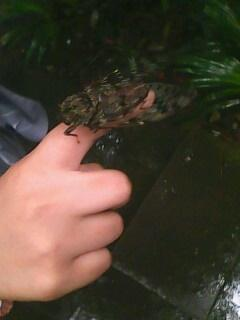
\includegraphics[width=1in]{/home/bamboo/document/mynote/essay_cicada.jpg}
\title{蝉}
三年地下生,今夕破土爬出来。
展翅可扑高枝,鼓膜能扬远声,悠然自在真了不得。
惜哉命不长,力微声短,无可奈何,但求一处息。

你把露珠看得越清楚,它旁边的花草就变得越模糊.亲近一个人必然疏远其他人,亲近于人必然疏远于自然.远离人情才能看到真理.\date{2012.10.27}

我等待着和你见面,就想跟你说一句话。我只是呆呆地看着时间流走,尽管我知道一见到你我将什么也说不出口。\date{2012.11.7}

我最关心的人是你,因为你是最关心我的人,但是我并不奢求你最关心的人是我,也不敢去想我是最关心你的人。\date{2012.12.14}

乐莫乐于相知兮,伤莫伤于相忘。奈何相忘且多兮,相知且易逝。于是说,虽则海枯石烂,其人心不变。
\date{2013.3.6}

曾经,我不认识你,你也不认识我。后来,你认识了我,我也认识了你。其实,我不必认识你,你也不必认识我。然而,我时刻想念你,你时刻被我想念。终于,我爱上了你,你却不接受我的爱。
\date{2013.8.26}

\title{班委竞选讲稿}
首先感谢两年来大家对我的支持,并非第一次参加班委竞选,心情反而更加激动。我这次要单选的职务是团支书。想到这个职务,深感责任重大,丝毫不敢怠慢;又深感不足,必须努力提高。

这是大学的第三年,相当于现在的早秋时节,对很多人来讲,这是十分关键得以操纵命运的一年。因此,当班委是有重大意义的,此所以我又一次走上竞选的讲台,在竞选的名单上写下自己的名字。

我于班委所想的关乎大家的有三点:一是情感,要有融恰的班级气氛,深厚的同学情谊,让我们的班级更象一个集体;二是成绩,同学们在考虑前程的时候,还会发现,成绩或者奖学金是不容轻视的,因此提高成绩是班委的一大任务;三是就业准备,如今就业形式不容乐观,我们必须精心准备,好让眼光长远些,机遇更大些,这需要大家互相帮助。

如果我竞选团支书成功,向大家保证:一定认真负责,积极主动,不偏心,不利己,带领大家走向期望的生活。请投我一票,谢谢。
\date{2013/9/4}


\title{河边草}
\begin{verse}
河边草,青啊青。路边花,红啊红。\\
微风轻拂娇嫩柳,斜日暖照麦光莹。\\
车行过处飞尘土,孩童追逐留欢声。\\
芒芒星光夜未尽,总归还是故乡情。\\
\end{verse}\begin{verse}
河边草,青又青;树上鸟,鸣又鸣。\\
细雨斜飘东风起,低云渐遮皎月明。\\
寒冬孤寂思春归,醉卧春怀舍一生。\\
心中多少悔恨事,直欲时钟逆向行。\\
\end{verse}\date{2013.12.20}

\title{《鸟和青蛙》读后感}
同是以食虫为生,你是鸟还是青蛙呢?

 鸟飞到高处,俯瞰领域的远景。
 青蛙在泥地里,只看到周围的花草。
鸟喜欢把不同领域的问题整合起来,规划辽阔壮观的远景,以引领新方向。
青蛙每次只思考一个问题,澄清错综复杂的细节,以把基础夯实。
在数学中,也是在许多其他领域中,既需要鸟,也需要青蛙。
鸟有锐利的眼睛,
而青蛙有长长的舌头。
鸟飞过丛林,错过了许多鲜美的虫子,
青蛙细心地等待猎物,不知道更多的虫子在别处。

我希望自己是一只鸟,不料却变成了青蛙。
\date{2013.12.28}

\title{什么是爱情}
什么是爱情,为什么会爱一个人?
如果所爱的人变了,你还一如既往地爱她吗?
我将回答会。
既然如此,爱一个人不是因为她的任何特征,而仅仅是她本身。
因此,你的爱不是针对某个人,而是一种意识,
爱的意识加在你所爱的人身上,是你爱她的唯一原因。
如果你把这种意识加在另一个人身上,你也会同样地爱这个人,
而且是毫不保留地。
你要问:那岂不是把另一个人当成原先爱的人了吗?
不!因为所爱的人的变化不影响你爱她,
所以你的爱里不存在爱人的一切,
那么转移到另一个人身上的也只有纯净的爱。
这时候你可以回答:爱情是一种纯净的意识,相同的爱可以给不同的人。
这样,经过我的论证,爱情的适用性得以提高。
恋爱的人分手和结识新欢将会在更快的时间内完成,
因为所爱的不是一个人,而是自己脑子里的若干细胞。
\date{2014.2.10} 

\title{你会不会写这样的一封信}
\begin{verse}
你会不会写这样的一封信?\\
明知道收信人会把它扔掉。\\
千言万语,注定只是徒劳。\\
有痴心者,把想说的话语,\\
全部都写出来,并且说道,\\
就算被丢弃,也心甘情愿。\\
然后真真地以为她会看到,\\
岂肯信她转手就将信儿抛。\\
有痴情者,把所有的话语,\\
都藏在心底,站在高楼上,\\
静静地望着春风等待时机。\\
只是不相信,冬天到来时,\\
想说的话儿,半句未出口。\\
如果是你,\\
告诉我,该怎么办。\\
\end{verse}\date{2014.2.24}


%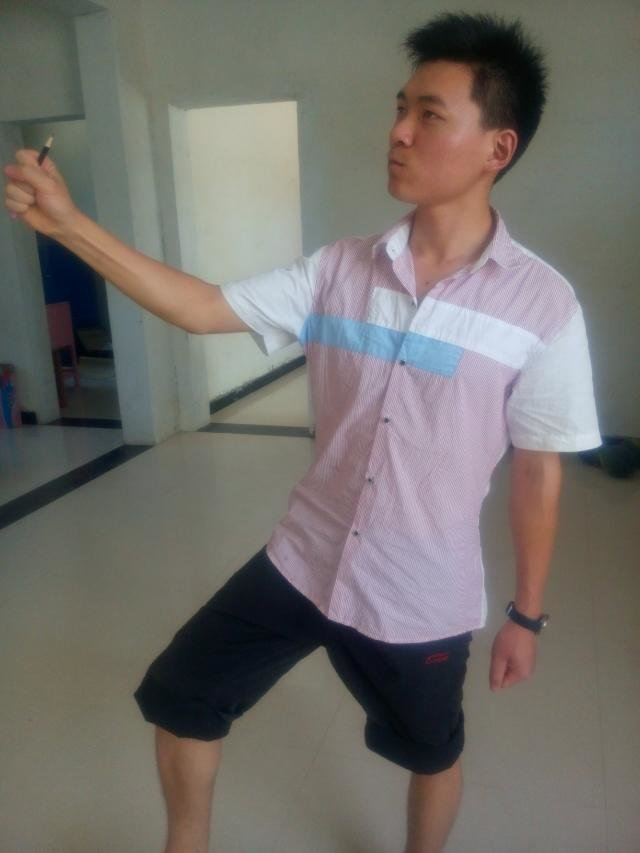
\includegraphics{/home/bamboo/document/mynote/essay_pipeful}
斗方名士兮,孤芳自赏。高视阔步兮,昂昂乎不可一世。

%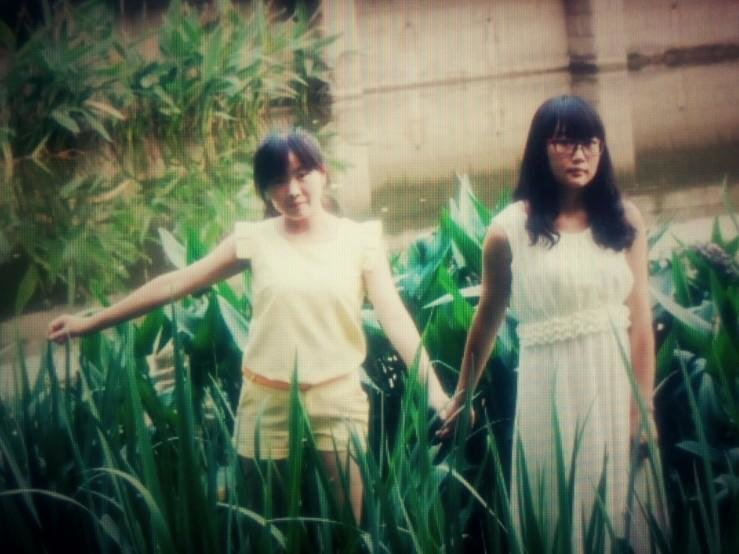
\includegraphics[width=1in]{/home/bamboo/document/mynote/essay_butterfly.jpg}
短衫与长裙,追逐蝴蝶飞。
蝴蝶双双去,我亦把家回。
前行莫急急,光阴且莫催。
待我一挥手,哪知作别谁?

\title{仙之人兮王崇宁}
仙之人兮王崇宁,驾龙上升兮入太清。\\
步玉屐兮执蕉扇,渺渺白云兮身无形。\\
勿谓我兮在梦中。
\date{2014.8.13}

\title{信封上的回忆}
什么都不想说了。\\
我只是不明白,不明白我自己。\\
半年前写给你的那封信,为什么现在还留在我手里?\\
我曾日日把它带在身边,为什么始终没有把它送给你?\\
或许是胆怯,或许是心虚。\\
但当我见不到你时,却非常希望我拿着它与你相遇。\\
我确信自己不是一个邮递员,\\
 在有机会给你的时候犹犹豫豫。\\
我确信又是一个邮递员,\\
 在想打开它的时候忽觉封印神圣不可欺。\\
谁肯信浇灭我拆开它的冲动的理由,\\
 竟是那样地简单那样地美丽:\\
我宁愿忘记信中一切的内容,也要记得自我封上它的那时起就期待着你打开它的那一刻。
\date{2015.3.8}
\end{document}
